\chapter{Methods}

We now develop a method for calibrating model parameters for a \emph{P. vivax}
model. In order to validate the method we create a simulation study. This is
where we simulate our observed data from the model, and then use that data
to recover the parameters used in creating our observed data.

\section{Creation of Synthetic Data}

\begin{figure}[htbp]
    \centering
    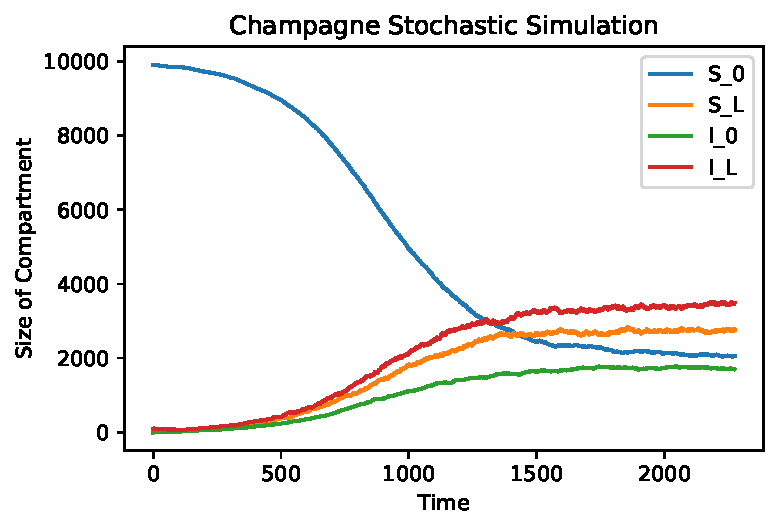
\includegraphics[width = \textwidth]{
        ../champagne_GP_images/champagne_simulation.pdf
    }
    \caption{
        A Doob-Gillespie Simulation of the model described by
        \cite{champagne_using_2022} with $\alpha = 0.4,$ $\beta = 0.4,$
        $\gamma_L = 1 / 223,$ $\lambda = 0.04,$ $f = 1 / 72,$ $r = 1 / 60,$ and
        $\delta = 0.$ The population was 10000, with 100 initial infections
        (both blood and liver stage $I_L$).
    }
    \label{fig:champ_doob}
\end{figure}

\begin{table}[htbp]
    \caption{
        The parameters used to simulate a \textit{P. vivax} outbreak using
        the model described by \cite{champagne_using_2022}
    }
    \label{tab:synth_params}
    \centering
    \begin{tabular}{c | c | c | c}
        Parameter description                      & Parameter
                                                   & Value      & Units     \\
        \hline
        effective blood stage treatment proportion & $\alpha$
                                                   & $0.1235$      & None      \\
        effective liver stage treatment proportion & $\beta $
                                                   & $0.429$      & None      \\
        rate of liver stage disease clearance      & $\gamma_L$
                                                   & $1 / 383$  & $1/$days  \\
        rate of infection                          & $\lambda$
                                                   & $0.01$     & $1/$days  \\
        rate of relapse                            & $f$
                                                   & $1/69$     & $1/$days  \\
        rate of blood stage disease clearance      & $r$
                                                   & $1/60$     & $1/$days. \\
    \end{tabular}
\end{table}

We investigated the model by \cite{champagne_using_2022} as described in 
Section
\ref{sec:champ_mod}. A malaria epidemic was simulated using the Doob-Gillespie
algorithm shown in Figure \ref{fig:champ_doob}, using a population
size of 10,000, and initial infected population of 100 (with both liver and blood
stage infection). The parameters used closely followed those reported in
\cite{champagne_using_2022}, with the exact parameters used reported in Table
\ref{tab:synth_params}. To simplify our analysis, we have assumed that case
importation is negligible, and therefore we have set $\delta = 0.$
From initialisation, the simulation was run for 200,000 time steps, 
after which, the model was
assumed to have reached steady state behaviour. 
The number of time steps was chosen as the stopping criteria,
because the time the model takes to reach a steady state is highly dependent 
on the scales of the parameters. Time steps adapt with the scale of
the parameters.

\begin{table}[htbp]
    \caption{
        Observed synthetic data
        $\by^\obs := \{\iota_\text{obs}, \pi_\text{obs}, i_\text{obs}, p_{obs}\}$
        from the simulation in Figure \ref{fig:champ_doob}.
    }
    \label{tab:obs_data}
    \centering
    \begin{tabular}{c|c|c}
        Parameter Description                        & Parameter
                                                     & Observed Value     \\
        \hline
        Weekly incidence at epidemic steady state    & $\iota_\text{obs}$
                                                     & 461                \\
        Prevalence at epidemic steady state          & $\pi_\text{obs}$
                                                     & 5205               \\
        Incidence in the first month of the epidemic & $i_\text{obs}$
                                                     & 42                 \\
        Prevalence after one month of the epidemic   & $p_{obs}$
                                                     & 87                 \\
    \end{tabular}
\end{table}


Within our assumed model framework, 
new infections which instantly undergo radical cure do not change the size of
each compartment. These infections should contribute to our incidence, 
even though they are not calculated. To account for this, silent infections, 
we calculated the number of additional infections to be 
Poisson distribution with rate
$\Delta t \times \alpha \beta \lambda (I_L + I_0) S_0 / N,$ where $\Delta t$ is
the time between events (one time step).
The (simulated) observed data was taken to
be from the simulated case counts (incidence) and prevalence
(as the absolute number of people infected) of the
simulated epidemic, described in Table \ref{tab:obs_data}.

\section{Model Simulations and Discrepancy Function}

New epidemics were simulated as above, with 200,000 events and at least 30
days (to allow for calculation of incidence in the first month of the
epidemic), with parameters
$\btheta = \{\alpha, \beta, \gamma_L, \lambda, f, r\}$
For each model
$y(\btheta) = \{\iota, \pi, i, p\}$ was
calculated with the same method as $\by^\obs,$ where the interpretation of each
parameter is described in Table \ref{tab:obs_data}.

We defined the discrepancy function to be $L_2$ norm of the relative
differences
$$
    \D(\btheta) = \D(\alpha, \beta, \gamma_L, \lambda, f, r)
    := \sqrt{
        \left(\frac{\iota - \iota_\text{obs}}{\iota_\text{obs}}\right)^2
        + \left(\frac{\pi - \pi_\text{obs}}{\pi_\text{obs}}\right)^2
        + \left(\frac{i - i_\text{obs}}{i_\text{obs}}\right)^2
        + \left(\frac{p - p_\text{obs}}{p_\text{obs}}\right)^2
    }.
$$
Relative difference was chosen to limit the impact between the scale
differences of the summary statistics.

\section{Gaussian Process and Initialisation}

We approximated $\E[\ln\D(\btheta)]$ with
a Gaussian process $d_\GP(\btheta)$ surrogate model.
$d_\GP(\btheta)$ was regressed on sample means
$$
    \smtheta := \frac{1}{30}\sum_{j = 1}^{30} \ln\D_j(\btheta)
$$
where the $\ln\D_j(\btheta)$s are i.i.d.\ samples generated by model runs.
Each evaluation of the discrepancy function was run in parallel 
using a supercomputer.
The samples
$\smtheta$ were assumed to be noisy observations of
$\E[\ln\D(\btheta)] + \varepsilon,$ where
$\varepsilon \sim N(0, \sigma_o^2),$ by the central limit theorem.
$\sigma_o^2$ was assumed to be independent of $\btheta,$ and has the natural
interpretation as the variance of the sample mean.
$d_\GP(\btheta)$ was assumed to have unknown constant mean $m_\GP$, and kernel
$$
    k(\bm{\theta}_i, \bm{\theta}_i^\prime)
    = \sigma_k^2 (1 + z_i + \frac{z_i^2}{3})\exp(-z_i)
$$
where
$$
    z_i = \sqrt{
        5 \sum_{\theta\in \bm{\theta}}\left(
        \frac{\theta_i - \theta_i^\prime}{\ell_\theta}
        \right)^2
    }.
$$
This kernel is, a Mat\'ern kernel with $\nu = 5/2$ and automatic
relevance determination - i.e.\ each parameter $\theta\in\btheta$ was
scaled by $\ell_\theta.$ In effect, this assigns each parameter its own
length hyperparameter. It is important that each parameter has its own length
scale because each parameter has different scales, and has varying degrees of
impact on the mean of the log discrepancy.

\begin{table}[htbp]
    \caption{
        Conservative upper bounds for parameters to be calibrated.
        Values were informed by
        \cite{champagne_using_2022, white_variation_2016}. All lower bounds
        were zero.
    }
    \label{tab:param_bounds}
    \centering
    \begin{tabular}{c |c |c}
        Parameter
         & Upper Bound & Unit   \\
        \hline
        Proportion of treatment clearing blood stage disease $\alpha$
         & 1           &        \\
        Proportion of treatment clearing liver stage disease $\beta$
         & 1           &        \\
        Rate of liver stage disease clearance $\gamma_L$
         & 1/30        & 1/days \\
        Rate of infection $\lambda$
         & 1/10        & 1/days \\
        Rate of relapse $f$
         & 1/14        & 1/days \\
        Rate of blood stage disease clearance $r$
         & 1/14        & 1/days
    \end{tabular}
\end{table}

All parameters to be calibrated were given conservative upper bounds after
considering values reported in the literature. $d_\GP(\btheta)$ was fit
over this compact subspace of the whole parameter space.

\begin{table}[htbp]
    \caption{
        Hyperparameters used in training $d_\GP(\btheta).$
    }
    \label{tab:hps}
    \centering
    \begin{tabular}{c|c}
        Hyperparameter    & Description                                \\
        \hline
        $\sigma_k^2$      & Mat\'ern kernel amplitude                  \\
        $\sigma_o^2$      & Observation variance ($\var(\smtheta)$)    \\
        $\ell_\alpha$     & Length parameter associate with $\alpha$   \\
        $\ell_\beta$      & Length parameter associate with $\beta$    \\
        $\ell_{\gamma_L}$ & Length parameter associate with $\gamma_L$ \\
        $\ell_\lambda$    & Length parameter associate with $\lambda$  \\
        $\ell_f$          & Length parameter associate with $f$        \\
        $\ell_r$          & Length parameter associate with $r$        \\
        $m_\GP$           & Gaussian process mean
    \end{tabular}
\end{table}

Latin hypercube sampling was used to initialise 50 samples of the
parameter space (scaled to be between zero and the upper bounds described in
Table \ref{tab:param_bounds}). For each set of parameters,
$\smtheta$ was generated. The hyper\-parameters described in Table \ref{tab:hps}
were optimised using leave one out cross validation of the log predictive 
likelihood described in
Equation \ref{eq:pred_log_prob}, and $d_\GP^{(0)}(\btheta)$ was
fit to the samples.

\section{Bayesian Acquisition and Parameter Updates}

\begin{algorithm}
    \caption{
        Gaussian process approximation of $\smtheta$ with Bayesian updating
    }
    \label{alg:GP_reg}
    \begin{algorithmic}
        \State \textbf{Input:} Initial values for $\btheta$,
        lower and upper bounds for $\btheta$,
        initial Gaussian process model $d_\GP^{(0)}(\btheta)$
        \State \textbf{Output:} Synthetic likelihood $\hat{L}(\btheta)$

        \For{$t = 1$ to $500$}
        \State
        $\btheta^{(t)} \gets \argmin_{\btheta} \mathcal{A}_\EI(\btheta)$
        \State Sample $\smthetat$
        \If{$t\leq 6$} \Comment{Once per parameter}
        \State $j \gets t$
        \State Create $\mathbf{s}_j,$ 15 evenly spaced values
        from 0 to the upper bound of $\theta_j$ in
        Table \ref{tab:param_bounds}

        \For{$k$ in 1 to 15}
        \State $\theta^{(t)}_j \gets s_{jk}$
        \State Sample $\smthetat$
        \EndFor

        \Else
        \State $j\gets t\mod 6$ \Comment{Iterating over $\btheta$}
        \For{4 repeats}
        \State Sample $U_j\sim \mathrm{Unif}(0, m_j),$ with $m_j$
        being $\theta_j$'s upper bound
        \State $\theta^{(t)}_j \gets U_j$
        \State Sample $\smthetat$
        \EndFor
        \EndIf

        \If{$t \mod 50 == 0$} \Comment{Every 50 iterations}
        \State Reoptimise the Gaussian process hyperparameters using
        leave-one-out cross validation
        \EndIf

        \State Update $d_\GP^{(t)}(\btheta)$ on the new samples
        \EndFor
        \State \Return $d_\GP^{(500)}(\btheta)$
    \end{algorithmic}
\end{algorithm}

The Gaussian process was optimised over 500 iterations. Each iteration involved
minimising the expected improvement and obtaining a new sample $\smtheta.$
For each iteration, one of the variables $\theta_j \in \btheta$ was chosen, and
multiple samples of $\smtheta$ were taken using multiple values for $\theta_j.$
This was in order to improve the values for the length parameters, but
also to explore the parameter space more widely. This step is highly
parallelisable.
The hyperparameters were
reoptimised every 50 iterations, as the number of samples increased. The full
procedure is specified in Algorithm \ref{alg:GP_reg}.

Given a the set of previously sampled parameters $\bTheta^\ast,$ and 
$\mu_* := \min_{\btheta^\ast\in\bTheta^\ast}\E(d_\GP(\btheta_\ast)),$
the expected improvement with exploration
$$
        \A_\EI(\btheta)
        := \E[\min(d_\GP(\btheta) - (\mu^\ast + 0.1), 0)],
$$
was minimised using a gradient descent algorithm. The gradient descent was
initialised at $\btheta^\dagger,$ where $\btheta^\dagger$ was a
combination of the best parameters yet observed
$\btheta^{**} := \argmin_{\btheta^\ast\in\bm{\Theta}^\ast} d_\GP(\btheta^\ast)$,
and values between 0 and the upper bounds described in \ref{tab:param_bounds}
distributed uniformly at random. Each $\theta_j^\dagger$ was set independently,
with
$$
    \Pr(\theta_j^\dagger = \theta_j^{**})
    = 1/2
    = \Pr(\theta_j^\dagger \text{ uniformly distributed}).
$$

We could have chosen random initialisation but we do not expect it to improve 
the algorithms success, because for samples where 
$\A_\EI(\btheta)$ is very small, particularly if
$d_\GP(\btheta^\ast)$ is
large, the gradient of $\A$ can be negligible, causing the convergence criteria
to be met prematurely.
Furthermore starting only at the current minimum will 
increase the possibility of being stuck in local minima.

The final fitted Gaussian process 
$d_\GP^{(500)}(\btheta)$ is an approximation of $\E(\ln\D(\btheta)).$ Since the
variance of the sample mean $\var(\smtheta)$ is estimated by $\sigma_o^2,$ the
variance of the the log discrepancy function $\ln\D(\btheta)$ is
approximately $30\sigma_o^2.$ We then used moment matching assuming that
$\D(\btheta)$ is approximately log-normally distributed
distribution, and hence can be approximated by
$$
    \hat{\D}(\btheta) \sim
    \LN\left(\E[d_\GP^{(500)}(\btheta)], 30 \sigma^2\right).
$$
Therefore using approximate Bayesian computation described in
Algorithm \ref{alg:abc}, the probability of sampling
and accepting a $\btheta$ is
$\Pr(\btheta)\Pr(\D(\btheta) < \epsilon | \btheta),$ where
$L(\btheta):=\Pr(\D(\btheta) < \epsilon | \btheta)$ approximates the true
likelihood $\L(\btheta).$
Finally, we substitute in our approximation $\hat{\D}$ for $\D,$ to create our
synthetic likelihood
\begin{align}
        \hat{L}(\btheta) := \Pr(\hat{\D}(\btheta) < \epsilon | \btheta).
        \label{eq:fin_lik}
\end{align}
Since
$$
    \ln\hat{\D}(\btheta)
    \sim N\left(\E[d_\GP^{(500)}(\btheta)], 30 \sigma^2\right),
$$
we can express $\hat{L}$ as
$$
    \hat{L}(\btheta) =\Pr(\ln\hat{\D}(\btheta) < \ln\epsilon | \btheta).
$$

This final step is the crux of our methodology. By recovering a likelihood
the standard frequentist and Bayesian methods for parameter estimation are 
once again usable.

The Gaussian process and Gaussian process regression was implemented using
TensorFlow \parencite{abadi_tensorflow_2015}, and all code
is available at \url{https://github.com/jaycrick/masters_project}.